%\documentclass[fleqn]{book}
\documentclass[11pt]{amsbook}

\usepackage[turkish]{babel}

%\usepackage{../HBSuerDemir}	% ------------------------
\usepackage{../Ceyhun}	% ------------------------
\usepackage{../amsTurkish}


\begin{document}
% ++++++++++++++++++++++++++++++++++++++
\hPage{220}
% ++++++++++++++++++++++++++++++++++++++
\newtheorem{thm}{Teorem}[section]
\newtheorem{defn}{Tanım}[section]
\begin{thm} i uygun biçimde ve yeterince
uygulayarak bir çizgenin, eğer varsa 1-ayrışımı
elde edilebilir. n-ayrısırlıkla ilgili genel bir
gerek ve yeter koşul veremeyiz. Ancak Euler
çizgelerinin 2-ayrışır olduğu kolayca görülebilir.
Şekil 4.4.3 de, D(7) nin 2-ayrışımı
gösterilmiştir.

	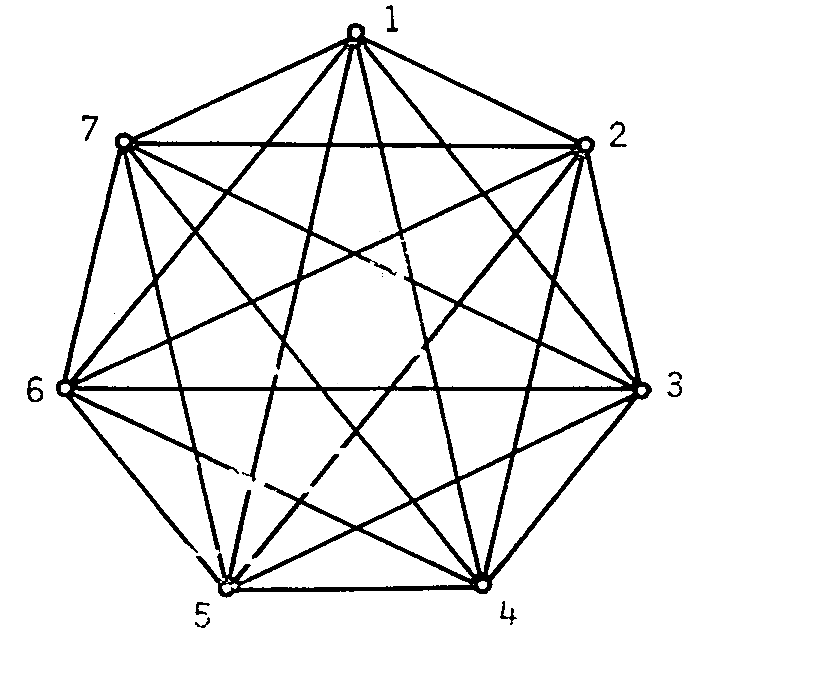
\includegraphics[width=0.45\textwidth]{images/Untitled2}
	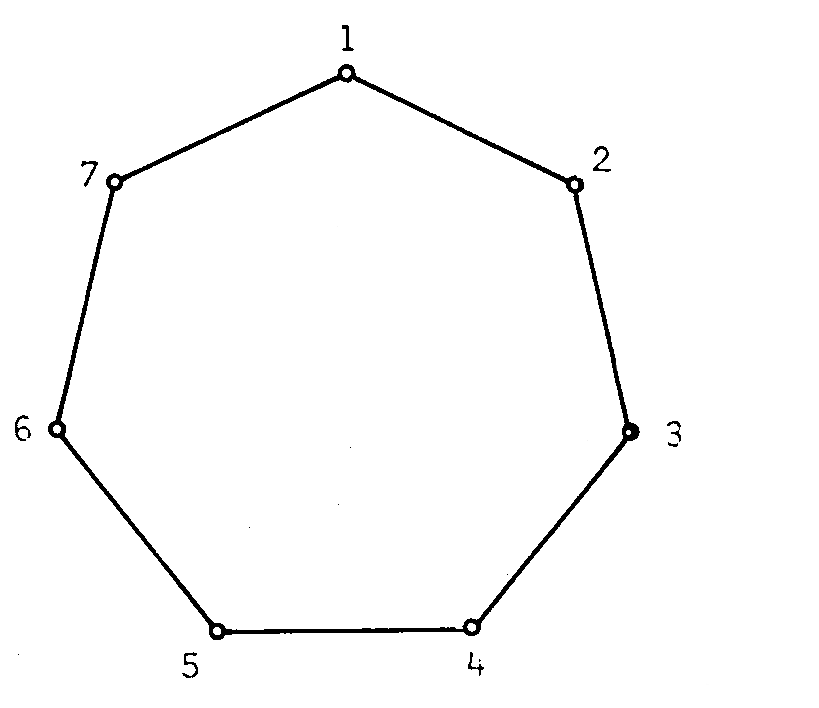
\includegraphics[width=0.45\textwidth]{images/Untitled}\\
	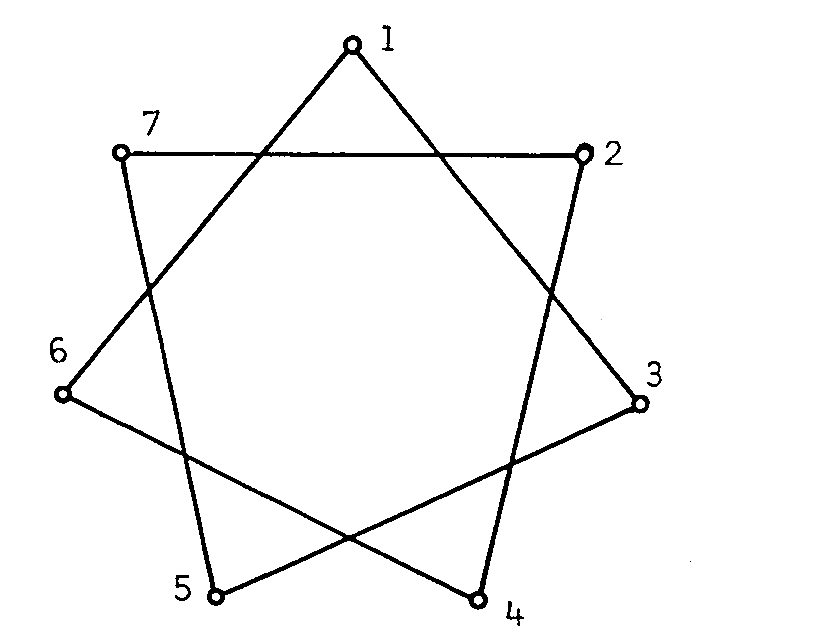
\includegraphics[width=0.45\textwidth]{images/Untitled3}
	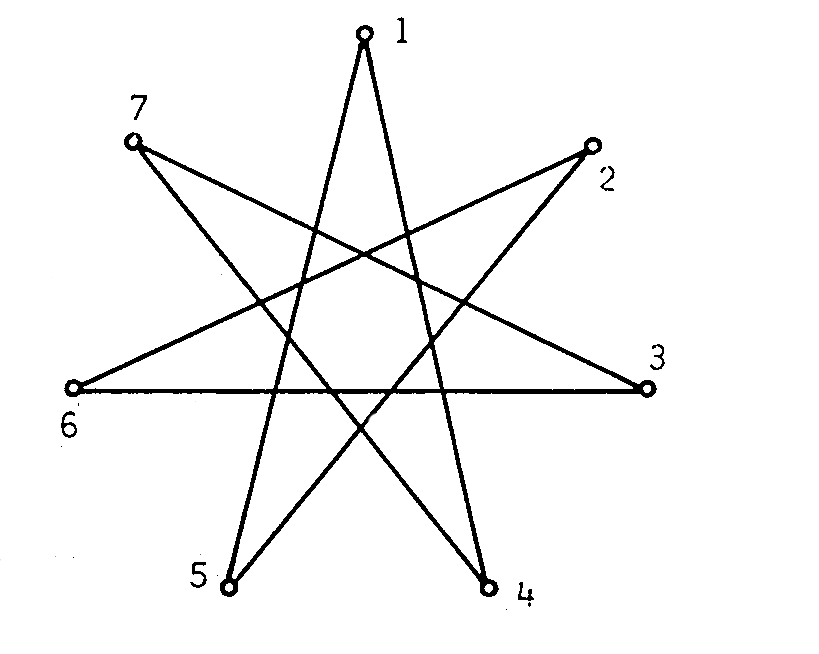
\includegraphics[width=0.45\textwidth]{images/Untitled4}
	\\
	Şekil 4.4.3 2-ayrısır bir çizge ve 2-ayrışımı.
	Başka bir ayrısım türü de, ağaç ayrışımıdır.
\end{thm}

\begin{defn}
$	z_i
$
 ve
 $ z_j, Ç(d,a)
$
 daki bütün düğümleri içeren iki Z-çizgesini
	göstersin. Bütün i ve j ler için,
$ Z_i \cap Z_j =\phi
$
koşulu altında, Ç(d,a) nın
ayrışabileceği en küçük kapsar
z-cizgesi sayısına çizgenin
\underline{ağaçlık katsayısı
$ \pi
$}
, bu ayrısmaya
da \underline{ağaç ayrışımı} denir.	
\end{defn}	

\end{document}